\documentclass[12pt]{report}
\usepackage{setspace}
\usepackage{amsmath}
\usepackage{amssymb}
\usepackage{xcolor}
\usepackage{subcaption}
\usepackage{float}
\usepackage{multicol}
\usepackage{graphicx}
\usepackage{parskip}
\usepackage{romannum}
\usepackage{authblk}
\usepackage[a4paper,margin=1in]{geometry}
\usepackage{times}
\usepackage{multicol}
\setlength{\columnsep}{1cm}
\usepackage{url}
\usepackage{titling}
\setlength{\droptitle}{-5em}
\singlespacing
\DeclareMathOperator*{\argmax}{argmax}

\begin{document}

\title{CS464 Introduction to Machine Learning \\ Homework Assignment 1} 
\author{Ilker Demirel}
\date{21502856}
\maketitle

\section*{Q1}
\subsection*{Q1.1}
Probability of any two students having same birthday in a classroom of size $n$ is (call this event, event $A$),

\begin{align} \label{eqn:q1}
P(A) &= 1 - P(A') \nonumber \\
&= 1 - \frac{365 \cdot 364 \dots \cdot (365 - (n - 1))}{365^n}
\end{align}

In equation (\ref{eqn:q1}), the denominator of the subtracted term is the total number of birthday combinations, and the nominator is the total number of birthday combinations when everyone student has a different birthday. See figure (\ref{fig:q1}) for $n$ vs $P(A)$.

\begin{figure}[h!]
  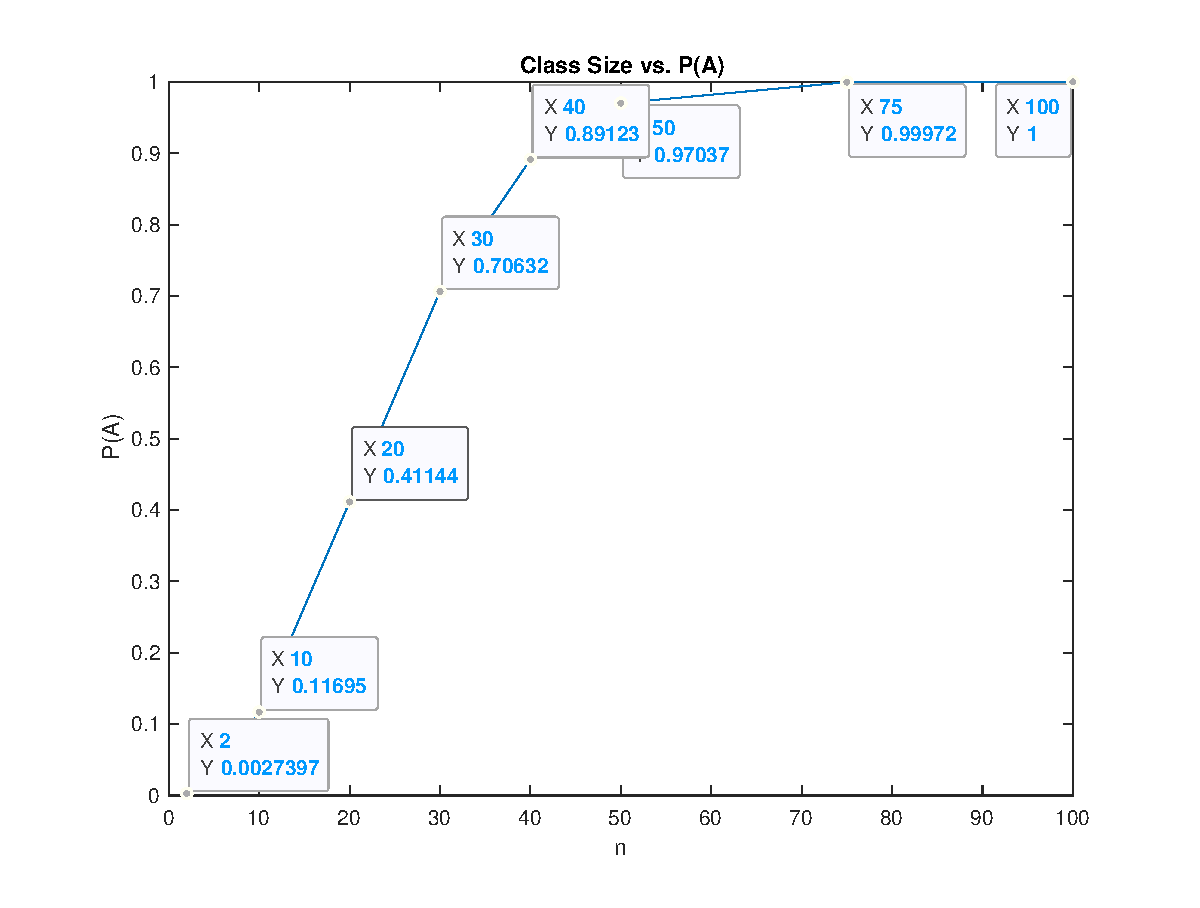
\includegraphics[width = \textwidth]{q1_1}
  \caption{Class Size ($n$) vs. $P(A)$}
  \label{fig:q1}
\end{figure}

\subsection*{Q1.2}
Minimum number of students to make sure that any two students have the same birthday is 366, since there are 365 days in a year.

\section*{Q2}


\subsection*{Q2.1}

$P(S=disease)~=$ 0.011 \\
$P(S=healthy)~=$ 0.989 \\
$P(T=positive|S=disease)~=$ 0.94 \\
$P(T=negative|S=disease)~=$ 0.06 \\
$P(T=positive|S=healthy)~=$ 0.02 \\
$P(T=negative|S=healthy)~=$ 0.98 

\subsection*{Q2.2}

$P(S=disease|T=positive)=\frac{P(T=positive|S=disease) P(S=disease)}{P(T=positive)}=\frac{0.94 \cdot 0.011}{0.94 \cdot 0.011 + 0.02 \cdot 0.989} \approx$ 0.35

Given the test result for a patient is positive, the probability that patient has the disease is 0.35. Therefore it is not reasonable to diagnose a patient with the disease when the test result is positive.

\subsection*{Q2.3}

Since $P(S=disease|T=positive) \neq$ 1, one can \textbf{never} definitely diagnose a patient as sick. That being said, the criterion for \textbf{confidentally} diagnosing a patient as sick is not defined in the question. Given there are $n$ positive test results, the probability that the patient is sick is,

\begin{align} \label{eqn:q2}
P(S=disease|n~positive~tests) &= 1 - 0.65^n
\end{align}

According to equation (\ref{eqn:q2}), if there are seven positive tests, the patient is sick with a probability of $1 - 0.65^7~\approx$ 0.95.

\section*{Q3}





\end{document}
